\chapter{Etat de l'art sur les attaques par prompt injection}
\vspace{2 cm}
%\section*{Introduction}
%\addcontentsline{toc}{chapter}{Introduction}
\section*{Introduction}
Prompt injection ou injection rapide, en cybersécurité, est une attaque qui vise les modèles d'apprentissage automatique, notamment les grands modèles de langage (LLM), en manipulant leurs instructions pour obtenir des comportements inattendus ou des réponses indésirables. Ces attaques exploitent l'incapacité du modèle à distinguer les instructions du développeur de celles de l'utilisateur, permettant ainsi aux attaquants de contourner les mesures de sécurité et d'influencer les sorties du modèle. 

Avec l’adoption massive des grands modèles de langage (LLMs) tels que ChatGPT, Claude ou Mistral dans les applications professionnelles, Les attaques par prompt injection (injection d’impulsion) sont une menace pour la sécurité de l’IA dans laquelle un attaquant manipule l’invite d’entrée dans les systèmes de traitement du langage naturel (NLP) pour influencer la sortie du système. Elles exploitent la manière dont les LLMs interprètent les requêtes textuelles (ou prompts) pour manipuler leur comportement, contourner des restrictions ou exfiltrer des données sensibles. Le terme « prompt injection » a été introduit pour la première fois en 2022 par Simon Willison, un chercheur indépendant et pionnier dans l’analyse des risques liés aux IA conversationnelles \cite{willison_prompt_nodate}. L’OWASP a classé ces attaques parmi les dix principales vulnérabilités à surveiller dans les applications exploitant des LLMs (OWASP Foundation, 2024)\cite{fasha_mitigating_2024}.

Face à l'accélération de l'adoption des IA génératives dans l'industrie et les administrations, la compréhension et la détection des attaques par prompt injection sont devenues une priorité pour les équipes de cybersécurité. Les systèmes LLMs sont de plus en plus intégrés dans des applications hautement critiques, des chatbots de service client aux algorithmes de trading financier, le potentiel d’exploitation augmente. Actuellement, nous assistons à un véritable jeu du chat et de la souris, dans lequel les utilisateurs tentent de détourner les modèles à l’aide des attaque par prompt injection, tandis que les développeurs essaient simultanément de découvrir les vulnérabilités et de bloquer ces attaques.

\section{types de prompt injections (injection rapide)}
	De manière générale, les injections de prompt peuvent être divisées en attaques directes et attaques indirectes. La principale différence réside dans l’endroit où l’injection est effectuée :
		\begin{itemize}
		\item \textbf{injection de prompt directes}, le prompt lui-même est modifié,
		\item tandis que dans les \textbf{injections de prompt indirectes}, c’est le contexte du prompt qui est manipulé
	\end{itemize}
	Ces deux types de prompt injection sont communs à toutes les ressources que nous avons visités tout au long de nos recherches. A partir des cette base, la \textbf{figure}\ref{fig1} obtenu de \cite{rossi_early_2024}, vas plus loin montrant qu'à partir de ses deux types, nous pouvons obtenir des dérivées en propasant un processus complet de catégorisation des différents type d'injections.
	\begin{figure}[h!]
		\centering
		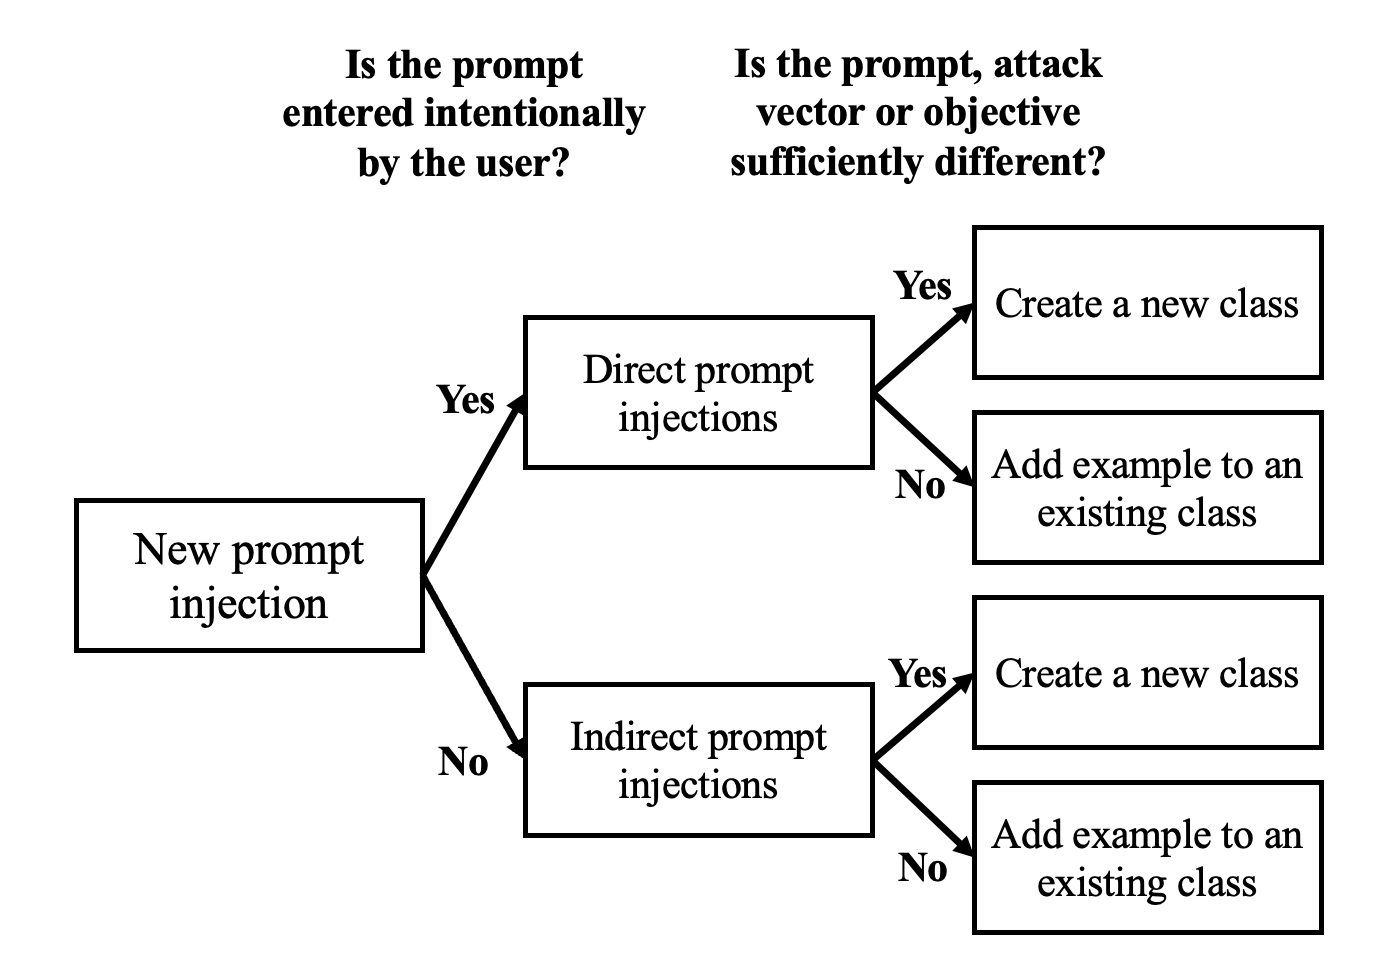
\includegraphics[width=0.7\linewidth]{img/process.png}
		\caption{processus de catégorisation}
		\label{fig1}
	\end{figure}
	
\subsection{Prompt injection indirecte}
Injection de prompt indirect consiste à cacher dans une source externe, par exemple une page web, un fichier PDF ou une image qui sera analysée par le LLM. C'est le cas des attaques multimodales, où des messages malveillants sont encodés dans des visuels. Dans ce type d'attaque, les attaquants influencent progressivement le comportement du système au fil du temps en insérant des invites malveillantes dans les pages Web que les attaquants savent que le modèle consommera, modifiant subtilement le contexte ou l’historique de ces pages Web pour affecter les réponses futures \cite{mathew_enhancing_nodate}.

Les injections de prompt indirectes malveillantes peuvent avoir des objectifs bien plus néfastes, tels que l’exfiltration de données depuis un navigateur ou un e-mail vers un emplacement spécifié par l’attaquant (Burgess, 2023)\cite{burgess_security_nodate}. Le Tableau \ref{tab2} contient les descriptions et objectifs des prompt injections indirectes répertoriées dans \cite{rossi_early_2024}. La première classe, appelée injections actives, tire son nom du fait que l’attaquant tente proactivement de cibler des systèmes tels que des clients email augmentés par des LLM.
\begin{table}[h]
	\begin{tabular}{|l|p{6cm}|p{6cm}|}
		\hline
		\textbf{Injection Class} & \textbf{Description} & \textbf{Objective} \\
		\hline
		Active Injections & Malicious prompts that are actively delivered to an LLM, for examply by sending emails containing prompts so that an email client enhanced with an LLM extension executes the prompt. See example 14 in Appendix A. & Steal sensitive data and or provide an undesired output, or trick an LLM into running a malicious prompt. \\
		\hline
		Passive Injections  & Placement of malicious prompts or content inside a public source that might be read by an LLM. More broadly, it deals with the manipulation of data such as text on webpages evaluated by LLMs. See example 15 in Appendix A. & Trick an LLM into providing misinformation or into running a malicious prompt. \\
		\hline
		User-driven Injections & Sharing of seemingly innocent prompts using social engineering techniques, which then unwary users copy and paste into an LLM. See example 16 in Appendix A. & Trick an unsuspecting user into entering a malicious prompt. \\
		\hline
		Virtual Prompt Injection&The attacker manipulates the instruction tuning data of an LLM, so that so that in specific scenarios the model behavior is misaligned and provides outputs as is if was given additional instructions through a prompt. See example 17 in Appendix A. & Make an LLM to behave in a way desired by the attacker, such as produce biased outputs.\\
		\hline
	\end{tabular}
	\caption{\underline{Indirect prompt injections}}
	\label{tab2}
\end{table}	
\subsection{Prompt injection directe}
	une attaque par prompt injection se produit lorsque l’utilisateur fournit une instruction malveillante directement dans le prompt, avec l’intention de faire ignorer les instructions du système \cite{noauthor_securing_2023}.
	
	Les prompt injections directes ont le plus souvent un objectif simple : contourner les mesures de sécurité qui empêchent la génération de certains types de contenus.
	Parmi les actions généralement interdites figurent la génération de discours haineux, de malwares, de contenus incitant à la violence ou à des activités illégales, ou encore de contenus pour adultes\cite{rossi_early_2024}.
	
	Un autre objectif connu des injections de prompt directes peut être d’amener l’interface LLM par exemple un chatbot utilisant une API de LLM à révéler son “prompt initial”, c’est-à-dire les instructions qu’il a reçues.
	
	La majorité des articles que nous avons rencontré se concentre plus sur les prompts injections directes. Cela est probablement dû à la facilité avec laquelle elles peuvent être testées et démontrées, notamment avec des modèles comme GPT-3, ChatGPT ou Bing AI. Le tableau\ref{tab1} obtenu de \cite{rossi_early_2024} expose les différentes classes d'injections directes et founit une description de chaque classe et l'objectif spécifique de chacune.
	\begin{table}[h]
		\begin{tabular}{|l|p{6cm}|p{6cm}|}
			\hline
			\textbf{Injection Class} & \textbf{Description} & \textbf{Objective} \\
			\hline
			 Double character & A prompt that makes the LLM produce a double character response, with one character constrained by the language model’s rules while the other character is unconstrained and bypasses content restrictions. Some sources refer to these as jailbreaks. & Bypass security measures in LLM interfaces and produce malicious outputs. \\
			\hline
			Virtualization & A prompt that puts the LLM into an unrestricted mode, such as a developer mode or a virtual scenario where the malicious content is generated inside a ”virtual machine”. Some sources refer to these as jailbreaks. & Bypass security measures in LLM interfaces and produce malicious outputs. \\
			\hline
			Obfuscation & A prompt that has malicious content or rule-breaking instructions obfuscated, for example, by being encoded as base64 characters rather than regular ASCII characters. & Bypass security measures in LLM interfaces and produce malicious outputs. \\
			\hline
			Payload Splitting & Multiple prompts contain instructions that are combined with a final prompt. For example, when text A and text B are benign alone but malicious when combined into text A+B. & Bypass security measures in LLM interfaces and produce malicious outputs.\\
			\hline
			 Adversarial Suffix & A computationally generated suffix that looks like a random set of words and characters that is added to a malicious prompt, which circumvents the alignment of the LLM and results in a response to a malicious prompt. & Bypass security measures in LLM interfaces and produce malicious outputs.\\
			\hline
			 Instruction Manipulation & A prompt that either reveals the pre-written instructions or the initial prompt given to the interface of the LLM or a prompt that instructs the interface to ignore these instructions. & To reveal the LLM interface’s setup and or to modify it to allow producing malicious outputs.\\
			\hline
		\end{tabular}
		\caption{\underline{Direct prompt injections}}
		\label{tab1}
	\end{table}

	
\section{Protection contre les attaques par injection de prompt}
	Les attaques par injection de prompt representent une menace croissante pour les LLMs. Attaques directes ou indirectes, ces vecteurs d'attaque exploitent la manière dont les modèles traitent les instructions. Afin de renforcer la sécurité, plusieurs approches complementaires ont été proposées danns la litérature.
	\subsection{Défenses par prévention}
		La défense par prévention constitue un ensemble de méthodes identifiées dont l'objectif est de netoyer ou modifier les prompts avant leur exécution. on peut idenfier :
		\begin{itemize}
			\item le filtrage et l'encodage multiples, Zang et al. (2025) un schéma utilisant plusieurs encodages (Base64 par exemple) pour dissimuler les instruction malveillantes, assurant à la fois un faible taux d'échec et une bonne performance fonctionnelle\cite{zhang_defense_2025}.
			\item à cette méthodes s'ajoute le paraphrasage ou délimitation qui est une transformation du prompt (paraphrase, quotes, retokenization) a montré des résultats partiels pour casser les injections, mais reste insuffisamment fiable. Nous tirons le tableau \ref{tab3} dans \cite{zhang_formalizing_2025} qui montre pour chaque type de defense par prévention, la méthode à appliquée et la faiblesse de cette méthode.
			\begin{table}[h]
				\begin{tabular}{|l|p{6cm}|p{6cm}|}
					\hline
					\textbf{Défense} & \textbf{Méthode} & \textbf{Faiblesse} \\
					\hline
					Paraphrasage & Réécrit les entrées pour casser les injections. & Peut altérer le sens et réduire la précision.  \\
					\hline
					Rétokenisation & Découpe les mots en sous-unités (sous-mots) afin de perturber les attaques.& Permet toutefois à certaines injections de passer.\\
					\hline
					Délimiteurs & Encapsule l’entrée entre guillemets afin de séparer les commandes. & Ne bloque pas totalement les prompts injectés.\\
					\hline
				\end{tabular}
				\caption{\underline{Défense par prévention}}
				\label{tab3}
			\end{table}
		\end{itemize}
		
	\subsection{Défenses actives (alignment et fine-tuning)}
		Les défenses actives visent à renforcer la résilience des modèles de langage de grande taille (LLMs) face aux attaques par injection de prompt, non pas en bloquant simplement les entrées suspectes, mais en entraînant le modèle à reconnaître et rejeter activement les instructions malveillantes. Ce type de défense repose sur le renforcement de l’alignement entre le comportement du modèle et des principes de sécurité bien définis, notamment par des méthodes de fine-tuning supervisé ou auto-supervisé.
		\begin{itemize}
			\item la méthode SecAlign (Chen et al., 2024) repose sur un fine-tuning supervisé du modèle à l’aide de paires de données contenant à la fois des prompts sécurisés et des prompts malveillants (avec ou sans injection). L’objectif est d’apprendre au LLM à faire la différence entre un comportement attendu et un comportement dangereux, et à répondre de manière neutre ou refusée en cas de détection d’une injection.
			
			Les résultats expérimentaux de Chen et al. montrent que le modèle aligné via SecAlign réduit à presque 0\% le taux de réussite des attaques sur des scénarios variés, tout en maintenant une précision élevée dans les réponses aux prompts légitimes\cite{chen_secalign_2025}.
			\item le cadre SPIN (Self-supervised Prompt Injection Neutralizer) (Zhou et al., 2024), adopte une approche auto-supervisée, ne nécessitant aucune annotation manuelle. Il s’appuie sur une détection automatique des motifs d’injection dans le prompt à l’aide d’un réseau d’attention interne, suivi d’une neutralisation des segments suspects en temps réel, au moment de l’inférence\cite{zhou_spin_2024}.
			
			Contrairement à d'autres méthodes qui se contentent de bloquer ou modifier le prompt, SPIN tente de restaurer le prompt original en supprimant les injections détectées, puis autorise la réponse sur un prompt assaini. Cela permet d’éviter la perte d’information utile tout en réduisant la surface d’attaque.
		\end{itemize}
		
\section*{Conclusion}
	L’émergence des attaques par injection de prompt constitue un tournant majeur dans la sécurité des modèles de langage de grande taille (LLMs). Ces attaques, bien que récentes, exploitent une vulnérabilité fondamentale : la dépendance totale du modèle à son entrée textuelle pour déterminer son comportement. À travers cet état de l’art, nous avons distingué deux grandes catégories d’injection directes et indirectes chacune reposant sur des mécanismes d’exploitation spécifiques, souvent simples mais redoutablement efficaces.
	
	Les travaux recensés montrent que les techniques actuelles de prévention sont encore loin d’offrir une couverture complète. Des méthodes comme la rétokenisation, l’encapsulation via délimiteurs, ou encore la réécriture des prompts peuvent atténuer certains risques, mais elles présentent souvent des limites en matière de précision ou d’efficacité. De même, les approches de fine-tuning et d’alignement, bien qu’efficaces dans certains contextes, nécessitent des ressources importantes et une maintenance continue face à l’évolution des tactiques adverses.
	
	Ainsi, cet état de l’art nous a permis de comprendre la réalité critique : il n’existe pas à ce jour de solution unique et définitive contre les prompt injections. La protection des LLMs doit reposer sur une combinaison cohérente de techniques, à la fois algorithmiques, architecturales et humaines.